
\documentclass[conference]{IEEEtran}
% setup page to suit conference specification using fancyhdr
\usepackage{fancyhdr}
\setlength{\paperwidth}{215.9mm}
\setlength{\hoffset}{-9.7mm}
\setlength{\oddsidemargin}{0mm}
\setlength{\textwidth}{184.3mm}
\setlength{\columnsep}{6.3mm}
\setlength{\marginparsep}{0mm}
\setlength{\marginparwidth}{0mm}

\setlength{\paperheight}{279.4mm}
\setlength{\voffset}{-7.4mm}
\setlength{\topmargin}{0mm}
\setlength{\headheight}{0mm}
\setlength{\headsep}{0mm}
\setlength{\topskip}{0mm}
\setlength{\textheight}{235.2mm}
\setlength{\footskip}{12.4mm}

\setlength{\parindent}{1pc}


% If IEEEtran.cls has not been ins


\usepackage{graphics} % for pdf, bitmapped graphics files
\usepackage{epsfig} % for postscript graphics files
%\usepackage{mathptmx} % assumes new font selection scheme installed
%\usepackage{times} % assumes new font selection scheme installed
\usepackage{amsmath} % assumes amsmath package installed
\usepackage{amssymb}  % assumes amsmath package installed
\usepackage{subcaption}
\usepackage{multicol}



\hyphenation{op-tical net-works semi-conduc-tor}



 \setlength{\columnsep}{1.0cm}
 




\begin{document}

 \title{\fontsize{24pt}{10pt}\selectfont\textbf{OpenMotion}: An open source library for attitude estimation.} 

\author{\IEEEauthorblockN{Nizar Ouarti}
\IEEEauthorblockA{IPAL (Sorbonne UPMC, CNRS, \\Astar, NUS, UJF, IMT)\\
Singapore\\
Email: nizar.ouarti@ipal.cnrs.fr}
\and
\IEEEauthorblockN{Thomas Braud}
\IEEEauthorblockA{IPAL (Sorbonne UPMC, CNRS,\\ Astar, NUS, UJF, IMT)\\
Singapore\\
Email: braud.thomas@ipal.cnrs.fr }
\and
\IEEEauthorblockN{Vivien Billaud}
\IEEEauthorblockA{IPAL (Sorbonne UPMC, CNRS,\\ Astar, NUS, UJF, IMT)\\
Singapore }}

\maketitle

\thispagestyle{fancy}
\fancyhead{}
\lhead{}
\lfoot{}
\cfoot{}
\rfoot{}
\renewcommand{\headrulewidth}{0pt}
\renewcommand{\footrulewidth}{0pt}

\def\mathbi#1{\textbf{\em #1}}
\makeatletter
\newcommand*{\rom}[1]{\expandafter\@slowromancap\romannumeral #1@}
\makeatother






\begin{abstract}
The abstract goes here
\end{abstract}



\IEEEpeerreviewmaketitle

\section{Introduction}


\section{Global Presentation of the Library}






\begin{itemize}
\item The North East Down (NED) frame $\{a\}$ system has its origin fixed at the (moving) object center of gravity. The $z$-axis points upward perpendicularly to the tangent plane of the ellipsoid, and the $x$-axis points towards true north (and not the magnetic north). The $y$-axis point towards east.

\vspace{0.1cm}

\item The object-fixed reference frame $\{c\}$ is a moving and rotating coordinate frame that is fixed to the device. The $x$-axis points in the forward direction, the $y$-axis to the right side and the $z$-axis upward. 
\end{itemize}

We admit that all the components of the IMU belong to the same reference frame $\{c\}$ (ref figure~\ref{Schema_situation}). It is a cyclopean approximation \cite{ouarti2008multimodal} .

\begin{figure}[!h]
\centering
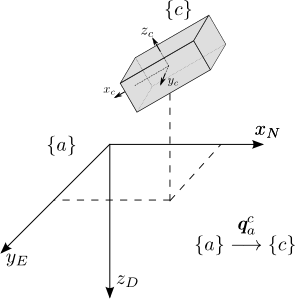
\includegraphics[scale=0.55]{images/Schema_situation.png}
\caption{Definition of the scene with 2 frame:  a fixed frame NED (North East Down) noted $\{a\}$ and a moving frame object noted $\{c\}$}
\label{Schema_situation}
\end{figure}


\section{Calibration and initialization}




\section{State of the art}

\subsection{Kinematic and quaternion representation}


A quaternion is a four-dimensional vector, defined as $ \mathbi{q} = \begin{pmatrix} \textbf{q} \\ q_w \end{pmatrix} $ with $ \textbf{q} =  ( q_x, q_y, q_z)^T $. For attitude representation, the quaternion must satisfies a single constraint given by  $|| \mathbi{q} || = 1$.The quaternion kinematics equation in discrete-time is given by :


\begin{equation}
\mathbi{q}_{k+1} = \Phi_{k+1|k}(\boldsymbol\omega)\mathbi{q}_{k}
\label{quat_kine}
\end{equation}

where $\boldsymbol\omega$ is the angular velocity and $\Phi_{k+4|k}$ is the transition matrix from time $k-1$ to $k$ such as:

\begin{equation}
 \Phi_{k+1|k}(\boldsymbol\omega) = \begin{pmatrix}  \cos(0.5||\boldsymbol\omega||\Delta T)I_3 - [\boldsymbol \psi\times] & \boldsymbol\psi \\ -\boldsymbol\psi^T &  \cos(0.5||\boldsymbol\omega||\Delta T)  \end{pmatrix} 
\end{equation}

 with,
 
\begin{equation}
 \boldsymbol \psi = \sin(0.5||\boldsymbol\omega||\Delta T)\frac{\boldsymbol\omega}{||\boldsymbol\omega||}
\end{equation}

And $[\textbf{v} \times] \in \mathbb{R}^{3\times 3}$ is the skew-symetric matrix of the vector $\textbf{v}$ such as.

\begin{equation}
[\textbf{v} \times] = \begin{pmatrix} 0 & v_z & -v_y \\ -v_z & 0 & v_x \\ v_y & -v_x & 0 \end{pmatrix} 
\label{skewsymmat}
\end{equation}
Then, the attitude matrix $R \in SO(3) $ related to the quaternion $\mathbi{q}$ is given by :

\begin{equation}
R(\mathbi{q}) = (q_w^2 - |\textbf{q}|^2)I + 2 \textbf{q}\textbf{q}^T - 2q_w[\textbf{q} \times]
\label{quat_to_rot}
\end{equation}

Where $SO(3)$ is the special orthogonal group defined by:

\begin{center}
$SO(3) = \{ R \in \mathbb{R}^{ 3 \times 3} | RR^T = R^TR = I, det(R) = 1 \}$
\end{center}


\subsection{Most Common Fusion Methods}


\subsubsection{Kalman Filtering Methods}


Introduced in 1960 by Kalman \cite{kalman_new_1960}, the Kalman filter is an algorithm that uses a series of measurements observed over time, containing noise, in order to estimate unknown variables (state vector). %The goal is to obtain more precise results than those based on a single measurement alone. 
Based on a model it is possible to obtain a more robust estimation of the state vector. Consider the following linear system, described by the difference equation and the observation model with additive noise:


\begin{equation}
\left\{ \begin{array}{l}
\textbf{x}_{k} = F_{k}\textbf{x}_{k-1}+B_{k}\textbf{u}_{k}+G_{k}\textbf{v}_{k}\\
\textbf{z}_{k} = H_{k}\textbf{x}_{k}+D_{k}\textbf{w}_{k}
\end{array} \right.
\label{linear_system}
\end{equation}

with,

\begin{center}
\begin{tabular}{rl}
$\textbf{x}_{k} $ &State vector at time $k$\\
$\textbf{z}_{k} $ &Measurement vector at time $k$\\
$\textbf{u}_{k} $ & Input vector (e.i.: from sensor) at time $k$ \\
$\textbf{v}_{k} $ & State noise vector disturbing the system\\
$\textbf{w}_{k} $ & Observation noise disturbing the measurement\\
\end{tabular}
\end{center}

\vspace{0.2cm}


The figure \ref{State_equation_discrete_case} represents the dynamical system described in \ref{linear_system} . A brief presentation of the algorithm is provided here,  see \cite{terejanu2013discrete} for more details. The algorithm has 3 important steps :\\



\begin{itemize}
\item The first step is the \textbf{prediction} of state $\textbf{x}^-_{k}$ at time $k$ and covariance $P^-_{k}$ is given by :

\begin{equation}
\left\{ \begin{array}{cl}
\textbf{x}^-_{k} = & F_{k}\textbf{x}^+_{k-1} + B_{k}\textbf{u}_{k} \\
P^-_{k} = & F_{k}P^+_{k-1}F^T_{k}+G_{k}Q_{k}G^T_{k}
\end{array}
\right.
\end{equation}

\item The \textbf{innovation} is the difference between predicted measurement and real measurement. It measure up the deviation used by the Kalman gain.
\begin{equation}
\left\{ \begin{array}{cl}
\boldsymbol\nu_{k} = & \textbf{z}_{k}-H_{k}\textbf{x}^-_{k} \\
S_{k} = & R_{k} +H_{k}P^-_{k}H^T_{k}
\end{array}
\right.
\end{equation}

\item And finally, An \textbf{update} is processed to correct the estimate state $\textbf{x}^+_{k} $ and his covariance $P^+_{k}$ with the innovation.

\begin{equation}
\left\{ \begin{array}{cl}
\textbf{x}^+_{k} = & \textbf{x}^-_{k} + K_{k}\boldsymbol\nu_{k} \\
P^+_{k} = &P^-_{k} - K_{k}S_{k}K^T_{k}
\end{array}
\right.
\end{equation}

\end{itemize}

Where $K_k$ is the Kalman gain  representing relative importance of innovation  $\nu_{k}$. 

\begin{equation}
K_{k}=P^-_{k}H^T_{k}S^{-1}
\end{equation}

%And so on for future state $k+1,...$. 




\subsubsection{Nonlinear Observer}

The theory of the state observer was first introduced by Kalman and Bucy for a linear system in a stochastic environment. Then Luenberger \cite{david1971introduction} made a general theory of observers for deterministic linear systems, introducing the notions of observer and reduced minimum observer \cite{primbs1996survey}. Mahony et al. \cite{mahony_nonlinear_2008} have proposed an nonlinear observer called Constant Gain Observer (CGO), termed the explicit complementary filter, that provides attitude estimates as well as gyro bias estimates. 

\begin{itemize}
\item Prediction
\end{itemize}

First, we propagate the estimate attitude and the gyro bias with equation \ref{prediction_cgo}.

\begin{equation}
\left\{\begin{array}{l}
\mathbi{q}_{k}^- = \Phi_{k|k-1}(\boldsymbol\omega_{gyro} - \boldsymbol \beta_{k-1}^+)\mathbi{q}_{k-1}^+ \\
\boldsymbol \beta_k^- = \boldsymbol \beta_{k-1}^+
 \end{array}
\right.
\label{prediction_cgo}
\end{equation}


\begin{itemize}
\item Correction
\end{itemize}


The idea is to compute a  constraint  given by a comparison between  an estimate value of a sensor and his real data at a time $k$. 

\begin{equation}
\left\{\begin{array}{l}
\textbf{v}_{acc}^- = R_(\mathbi{q}_{k}^-)\textbf{a}^a + \boldsymbol  \beta_{acc} \\
\textbf{v}_{mag}^- = R_(\mathbi{q}_{k}^-)\textbf{m}^a + \boldsymbol  \beta_{mag}
 \end{array}
\right.
\end{equation}

All these vectors are normalized. 

The '' gain '' is given by,

\begin{equation}
\boldsymbol \omega_{mes} = -vex(\sum_{i=1}^n \frac{k_i}{2}(\textbf{v}_i(\textbf{v}_i^-)^T -  \textbf{v}_i^-(\textbf{v}_i)^T )) 
\label{cgo_gain}
\end{equation}

where the $vex$ operator define by the inverse of the cross product.
\begin{equation}
\left\{\begin{array}{l}
\textbf{a}(\textbf{b})^T -  \textbf{b}(\textbf{a})^T  = [ (\textbf{a} \times \textbf{b}) \times ]\\
vex([\textbf{a}\times])  = \textbf{a}
 \end{array}
\right.
\end{equation}

Then, we the gain is used to correct the predicted attitude $\mathbi{q}_{k}^-$ by the following equation:

\begin{equation}
\left\{\begin{array}{l}
\mathbi{q}_{k}^+ = \mathbi{q}_{k}^- + \frac{\Delta T}{2} \Xi(\mathbi{q}_{k}^-) \boldsymbol\omega_{mes}k_p\\
\boldsymbol \beta_k^+ = \boldsymbol \beta_{k}^-  - \boldsymbol\omega_{mes}k_i
 \end{array}
\right.
\end{equation}

One problem of Kalman Filters is to find the initial values in the covariance (matrix $Q$) because it is difficult to relate it to real physical quantities. The covariance matrix is not involve in nonlinear observer theory. This is one of the reasons there has been an increasing interest for nonlinear observer design the last decades. Another reason is their low computational need.

\subsubsection{Methods Based on Solutions of the Wahba's Problem}

The attitude determination problem for vector observation was first formulated as a least squares estimation problem by Wahba \cite{wahba_least_1965} in 1965 :\\


Given the two sets of $n$ vectors $\{ \textbf{r}_{1},...,\textbf{r}_{n} \}$ and $\{ \textbf{b}_{1},...,\textbf{b}_{n} \}$, $n \geqslant 2 $, where each pair $(\textbf{r}_{i},\textbf{b}_{i})$ corresponds to a generalised vector, $\textbf{x}_{i}$, find the proper orthogonal matrix, $A$, which bring the first into the best least squares coincidence with the second. That is, find $A$ which minimises the function $J$ defined as:

\begin{equation}
J(A) = \frac{1}{2} \sum_{i=1}^n a_i||b_i-Ar_i||^2
\label{Wahba_loss_function}
\end{equation}

subject to the constraint $A^TA = I$ and $det(A)=1$. The equation (\ref{Wahba_loss_function}) can be written with a quaternion representation which gives:

\begin{equation}
J(\mathbi{q}) = \frac{1}{2} \sum_{i=1}^n a_i||b_i-R(\mathbi{q})r_i||^2
\label{QUEST}
\end{equation}

The matrix $R(\mathbi{q})$, is the rotation matrix that corresponds to the quaternion $\mathbi{q}$ (equation \ref{quat_to_rot}). The QUEST algorithm are conducted in the following manner. Let

\begin{equation}
B = \sum_{i=1}^N a_i\textbf{b}_i \textbf{r}_i^T
\end{equation}

Then, we can rewrite the equation (\ref{QUEST}) as follow

\begin{equation}
J(\mathbi{q}) = \frac{1}{2} \sum_{i=1}^n a_i  - tr(R(\mathbi{q})B^T)
\label{QUEST_bis}
\end{equation}

Due to the fact that the representation of the attitude matrix is a homogenous quadratic function of $\mathbi{q}$, we can say that

\begin{equation}
tr(R(\mathbi{q})B^T) = \mathbi{q}^TK\mathbi{q}
\label{QUEST_ter}
\end{equation}

where $K$ is the symmetric traceless matrix such as

\begin{equation}
K = \begin{pmatrix} S-tr(B)I_3 & \textbf{z} \\ \textbf{z}^T & tr(B)
\end{pmatrix}
\end{equation}

with

\begin{equation}
\left\{\begin{array}{l}
S = B + B^T\\
\textbf{z} = \sum_ia_i\textbf{b}_i\times\textbf{r}_i
 \end{array}
\right.
\end{equation}


The minimisation problem from Equation (\ref{QUEST_bis}) is now a maximisation problem. thus, the solution $\mathbi{q}_{opt}$ is the eingen vector correspond to the largest eigen value of $K$ \cite{markley1999estimate}. The main problem of QUEST is that it does not take into account of all the previous observations performed since the beginning. A recursive QUEST algorithm (REQUEST) proposed by Bar-Itzhack manages this problem. According to the REQUEST algorithm, the propagation of $K_k$ is given by

\begin{equation}
K_k^- = \Phi_{k|k-1}(\boldsymbol\omega_{gyro})K_{k-1}^+\Phi_{k|k-1}^T(\boldsymbol\omega_{gyro})
\end{equation}

We compute $\delta K_k $ as

\begin{equation}
\delta K_k = \frac{1}{\sum_ia_i}\begin{pmatrix} \delta S_k-\delta\sigma_kI_3 & \delta\textbf{z}_k \\ \delta\textbf{z}_k^T & \delta\sigma_k
\end{pmatrix}
\end{equation}

with,

\begin{equation}
\begin{array}{cc}
\delta B_k = \sum_i a_i \textbf{b}_i\textbf{r}_i^T & \delta S_k = B_k + B_k^T\\
\delta \textbf{z}_k = \sum_ia_i\textbf{b}_i\times\textbf{r}_i & \delta \sigma_k = tr(B_k)
\end{array}
\end{equation}

Where $\textbf{b}_i$ is the observation vector at time $k$. Then we update the K-matrix.

\begin{equation}
K_k^+ = \frac{\rho_k m_{k-1}}{m_k}K_k^- + \frac{1}{m_k}\delta K_k
\end{equation}


A drawback is that the value of $\rho_k$ comes from heuristics. Choukroun revisit REQUEST provides an improvement with his Optimal REQUEST \cite{choukroun_novel_2003} where an optimal $\rho_k^*$ is computed which gives better results. Here we choose to implement this version of REQUEST. Contrary to other methods, the QUEST algorithms do not estimate the gyroscope bias. Which can make it less robust in some cases.
There are also other methods based on Wahba's problem like the Davenport's q-method \cite{weighted1971nasa} proposed in 1971 considered more robust than QUEST. Or the method ESOQ proposed by Mortari \cite{mortari1997esoq}  in 1997. But in this study we limit our investigation to REQUEST.\\



\subsubsection{Particle Filtering Method}

Particle filtering method is based on Monte-Carlo method\cite{metropolis1949monte}. The main idea is to use a large number of samples called particles to estimate a nonlinear function \cite{chen_bayesian_2003} and \cite{terejanu2009tutorial}. The set of $N$ particle with associated weight at time $k$ are denoted by $\{\textbf{x}^{(i)}_{k},w^{(i)}_{k}\}$. Initially, the particle are drawn from a proposal distribution. The PF is divided into three step, prediction, update, resampling, that constitute a filter cycle:

\begin{itemize}
\item Prediction
\end{itemize}

The first step is to propagate all particles $\{\textbf{x}^{(i)}_{k-1},w^{(i)}_{k-1}\}$ to $\{\textbf{x}^{(i)}_{k},w^{(i)}_{k}\}$ with the nonlinear function $f$ while the weight remain unchanged : 

\begin{equation}
\textbf{x}^{(i)}_{k} = f(\textbf{x}^{(i)}_{k-1},\textbf{u}_{k-1}) + \textbf{w}_{k-1}^{(i)}\\
\end{equation}

where $N$ sample $\textbf{w}_{k-1}^{(i)}$ of the process noise (supposed gaussian in our case) are drawn.

\begin{itemize}
\item Update/Correction
\end{itemize}

At the update step, the weights associated with each particle is updated based on the likelihood function $p( \textbf{z}_k| \textbf{x}_k^{(i)})$.
\begin{equation}
\left\{ 
\begin{array}{l}
w_k^{(i)} = w_{k-1}^{(i)} p( \textbf{z}_k| \textbf{x}_k^{(i)})\\
\tilde{w}_k^{(i)} = \frac{w_{k}^{(i)}}{\sum_iw_{k}^{(i)}}
\end{array}
\right.
\end{equation}

The weight are normalised such as we have $\sum_i\tilde{w}_k^{(i)}=1$. To finish, the mean is computed with the following equation:

\begin{equation}
 \textbf{x}_k^+ = \sum_{i=1}^N\tilde{w}_k^{(i)} \textbf{x}_k^{(i)}
 \end{equation}



\begin{itemize}
\item Resampling/Regularisation
\end{itemize}

A common problem with PF is the degeneracy phenomenon. After some iterations, more and more particles will have a weak weight, which make them negligible and useless.  To overcome this problem, a regularisation step called resampling is processed. It is not needed to perform PF but it allows to maintain a good performance relative to degeneracy problem. The idea of resampling is to eliminate particles having feeble weight and focus on strong weight particles. In order to measure degeneracy, the number of effective samples $N_{eff}$ is computed (equation \ref{N_eff}). If  $N_{eff}$ is lower than a threshold, the resampling step is processed.

\begin{equation}
 N_{eff} = \sum_{i=1}^N\frac{1}{(\tilde{w}_k^{(i)})^2}
 \label{N_eff}
 \end{equation}


The choice of the threshold is important. Indeed, a high threshold gives $N_{eff} \approx N$, but that does not mean necessarily we have a lot of efficient particles. On the contrary, it means that most of the particle are identical making large computations unnecessary. Moreover, with a low threshold, many particles are neglected making computations less efficient. In general, the threshold is fixed at  $\frac{N}{2}$ or $\frac{N}{3}$.\\

There are several types of resampling, a comparison is made in \cite{douc2005comparison}. We took the resampling algorithm described in \cite{arulampalam2002tutorial} because it is the most commun. Cheng, Yang and Crassidis have propose an attitute estimation with a particle filter method \cite{cheng_particle_2010}. We have also considered the revisited algorithm of Cheng \cite{chang_particle_2014} based on bootstrap filter\cite{gordon1993novel}. We have chosen to implement this one because they use the same approach as USQUE \cite{crassidis_unscented_2003} and MEKF\cite{markley2003attitude}. We decided to explore the performance of this three algorithms with the same model. \\

The particle filter provides an estimate of the nonlinear system without assuming that the noise is Gaussian. So it is more robust to any situation, which makes it more performant in the context of a real applications. But an important computation time is required and that is a limitation for a real-time application.



\section{Performance Evaluation}


We have access through our designed ground truth to the true attitude $\mathbi{q}^{real}_k$ at time $k$ of the reference frame $\{c\}$ related to $\{a\}$.
By computation, each method returns an estimate attitude $\mathbi{q}^{est}_k$ at time $k$ (see figure \ref{test_method}). 

\begin{equation}
 \delta \mathbi{q}_k = \mathbi{q}^{real}_k \otimes (\mathbi{q}^{est}_k)^{-1} =  \begin{pmatrix}  \delta \textbf{q}_{k} \\ \delta q_{w_k}  \end{pmatrix}
\end{equation}

The error-MRP vector related to $ \delta \mathbi{q}_k$ is given by

\begin{equation}
 \delta \textbf{p}_k  = 4[\frac{\delta \textbf{q}_{k}  }{(1+\delta q_{w_k})}]
\end{equation}


Thus, we can calculate the attitude error given by the root mean square (RMS) of $\delta \textbf{p}_k$:

\begin{equation}
\epsilon_k  = RMS (\delta \textbf{p}_k) = \sqrt{\frac{1}{3}( \delta p_{k_x}^2 +\delta p_{k_y}^2+\delta p_{k_z}^2)  }
\label{error_definition}
\end{equation}

The mean of the error is given by :

\begin{equation}
\bar{\epsilon}  = \frac{1}{n}\sum_{i=1}^n \epsilon_i \\
\label{mean_var_error_def}
\end{equation}

With $n$ the number of data at our disposal. We use this information (mean error) for our performance study. 

\begin{figure}[!h]
\centering
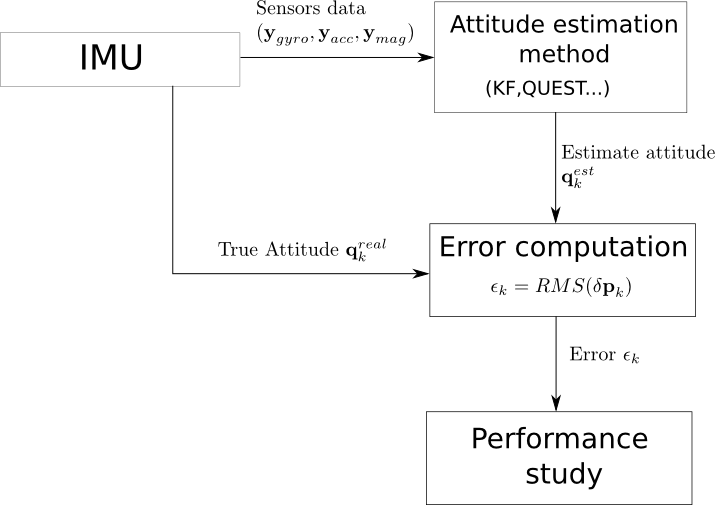
\includegraphics[scale=0.40]{images/test_method.png}
\caption{Algorithm designed to compute attitude estimation methods' performances}
\label{test_method}
\end{figure}


To differentiate the methods, we assigned  some ''scores'' in order to highlight the behaviour of these methods in different configurations. We defined these ''scores'' as:

\begin{align}
s_1 = \bar{\epsilon}\\
s_2 = \frac{1}{\bar{\epsilon} \times \bar{\tau}}
\label{score}
\end{align}

With $\bar{\epsilon}$ average attitude error (voir \ref{error_definition}) et $\bar{\tau}$ the average computation time. \\

\begin{figure}[!h]

\begin{subfigure}{.5\textwidth}
  \centering
  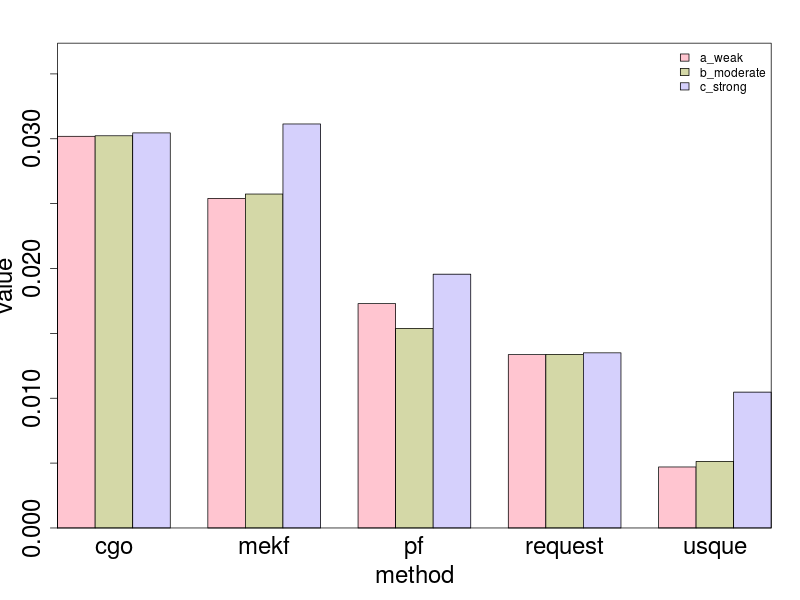
\includegraphics[width=.85\linewidth]{images/histo_s1_add.png}
  \caption{Mean Attitude Error (score $s_1$)}
\end{subfigure}%
\begin{subfigure}{.5\textwidth}
  \centering
  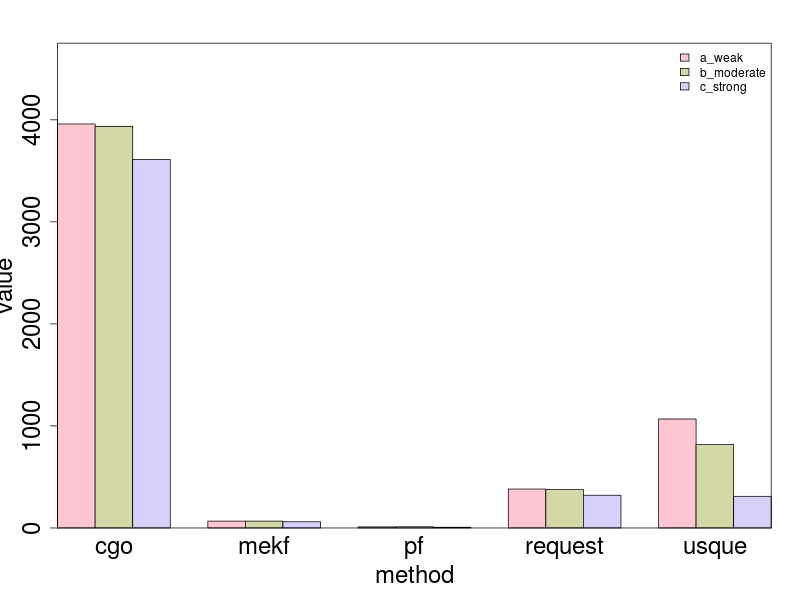
\includegraphics[width=.85\linewidth]{images/histo_s2_add.png}
  \caption{Ratio Error times Computation Time (score $s_2$)}

\end{subfigure}
\caption{Scores of methods where noise is AWGN with 3 strength}

\end{figure}


\section{Conclusion}

notre library est trop bien...

\bibliographystyle{ieeetr}


\end{document}